\documentclass[en]{../../../eplsummary}

\hypertitle{translators-INGI2132}{8}{INGI}{2132}
{Houtain Nicolas}
{Pierre Schauss}
$$$$

\section{Chapter 1}

\subsection{Compilation}

\subsubsection{Compilers}

A compiler is a program that \textbf{translates} a source program written in
a \textbf{high-level} programming language such as Java, C\# or C, into an
equivalent target program in a \textbf{lower level} language such as machine
code, which can be executed directly by a computer.

\begin{figure}[h]
    \centering
    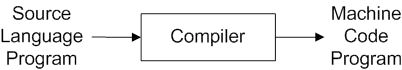
\includegraphics[width=8cm]{img/compilers.png}
    \caption{Compilation}
\end{figure}

\paragraph{Input $\to$ output} 
\begin{itemize}
    \item Mapping names to memory addresses, stack frame offsets and
        registers
    \item Generate linear sequence of machine code instructions
    \item Detecting any errors that can be detected
\end{itemize}


\subsubsection{Interpreters}
Interpreter executed directly th high-level language program.

\begin{figure}[h]
    \centering
    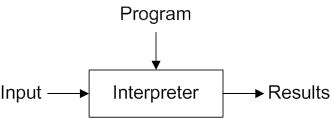
\includegraphics[width=8cm]{img/interpreters.png}
    \caption{Interpretation}
\end{figure}

\begin{enumerate}
    \item \textbf{Performance} : better with compilers (because
        interpreter must parse and analyse the statement ot decode its
        meaning \textit{every time} it execute that statement)
    \item \textbf{Secrecy} : more difficult to understand program with
        machine code
    \item[but] sometime, the overhead of interpretation doesn't always
        justify writing (or buying) a compiler. Like UNIX shell.
\end{enumerate}



\subsubsection{Programming languages}

Specified in three steps :
\begin{enumerate}
    \item \textbf{Tokens} : like work in natural language
    \item \textbf{Syntax}
    \item \textbf{Semantics}
    \item[Note] : The two first are described with formal notation, and
        the last is described with natural language.
\end{enumerate}

\subsubsection{Machines Languages}

A machine language program consists of a sequence of instructions and
operands, usually organized so that each instruction and each operand
occupies one or more bytes and so is easily accessed and interpreted.

A machine instruction set and its behavior is often referred to as its
\textbf{architecture}.

\paragraph{Note:} Java Virtual Machine (JVM) is said \textit{virtual}
because it is not necessarily implemented in hardware, rather it is
implemente as a software.

\subsection{Why study compilers}

\begin{enumerate}

\item Compilers are larger programs than the ones you’ve written
in your programming courses. It is good to work with a program that is
like the size of the programs you will be working on when you graduate.

\item Compilers make use of all those things you have learned about
earlier: arrays, lists, queues, stacks, trees, graphs, maps, regular
expressions and finite state automata, context-free grammars and
parsers, recursion and patterns. It is fun to use all of these in a real
program.

\item You learn about the language you are compiling (in our case, Java).

\item You learn a lot about the target machine (in our case, both the
Java Virtual Machine and the MIPS computer).

\item Compilers are still being written for new languages and targeted
to new computer architectures. Yes, there are still compiler-writing
jobs out there.

\item Compilers are finding their way into all sorts of applications
including games, phones and entertainment devices.

\item XML. Programs that process XML use compiler technology.

\item There is a mix of theory and practice, and each is relevant to the
other.

\item The organization of a compiler is such that it can be written in
stages, and each stage makes use of earlier stages. So, compiler writing
is a case study in software engineering.

\item Compilers are programs. And writing programs is fun.
\end{enumerate}




\subsection{Compiler work}
\begin{figure}[h]
    \centering
    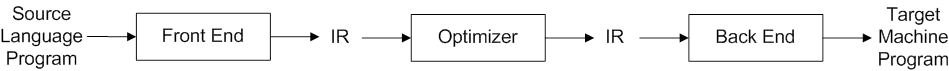
\includegraphics[width=8cm]{img/compilers_work.png}
    \caption{Compiler work}
\end{figure}

\subsubsection{Front end}
\begin{itemize}
    \item[-] Analyse the input program to determining its meaning
    \item[-] Source language dependent (target language independent)
\end{itemize}

\begin{figure}[h]
    \centering
    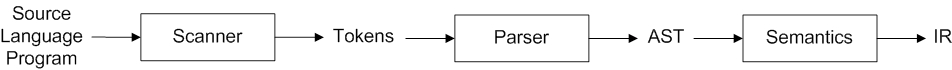
\includegraphics[width=8cm]{img/frontend.png}
    \caption{Front end : analysis}
\end{figure}

\begin{itemize}
    \item \textbf{Scanner} : With a input stream of character make a
        stream of tokens identifiers, literal, reserved word, operatos
        and separators
    \item \textbf{Parser} : Produce an abstract syntax tree (AST)
    \item \textbf{Semantics} : Declaring name in a symbol table, ,
    looking up names as they are referenced for determining their types,
    assigning types to expressions, and checking the validity of types.
\end{itemize}

\subsubsection{Back end}
\begin{itemize}
    \item[-] Produces a target machine program having the same meanig and is source 
    \item[-] Source language dependent (target language independent)
\end{itemize}

\begin{figure}[h]
    \centering
    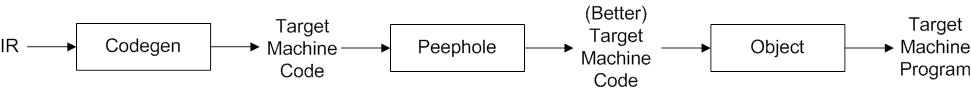
\includegraphics[width=8cm]{img/backend.png}
    \caption{Back end : analysis}
\end{figure}

\begin{itemize}
    \item \textbf{Codegen} : choosing what target machine instructions
        to generate. (information collected in earlier phases)
    \item \textbf{Peephole} : Generated instruction locallu for wasteful
        instructions sequences such as branches to branches and
        unnecessary load/stroe pairs.
    \item \textbf{Object} : Constructs a single machine code executable
        program
\end{itemize}

\subsubsection{Middle end}


\end{document}
